\chapter{Background Information on T Cells and Calcium Concentration}
\label{chapter:t-cell}

Lymphocytes form a key component of the immune system. T cells are a type of lymphocyte and are responsible for responding to viruses, fungi, allergens and tumours. Different subtypes of t cells exist, that perform various responsibilities. They are transported throughout the body via the lymphatic system and blood.\cite{Kumar2018}

Precursor cells are formed in the bone marrow. Once they are transported to the thymus they undergo maturation and selection to become t cells. Each cell forms receptors, called t cell receptors (TCR), that respond to one particular out of many ($10^6 – 10^9$) possible short pieces of proteins, called peptides. These peptides are attached to the major histocompatibility complex (MHC) present on antigens and antigen presenting cells (APC). Important aspects of the selection are ensuring that the t cells react to foreign peptides, but not to those present on the body's own cells.\cite{Ashby2024}

In positive selection, cells in the thymus present peptides on their MHC. If a t cell is unable to bind, it will undergo apoptosis, a type of cell death. T cells which were able to bind receive survival signals. Negative selection verifies that t cells will not attack the body's own cells. This is done by only selecting t cells which only bind moderately to the peptides presented, as a strong bond suggests that these t cells would have a high likelihood of being reactive to own cells.\cite{Hagel2018} If a t cell passed both the positive and negative selection it is transported to the periphery.

There are multiple types of peripheral t cells. Native t cells respond to new antigens. Cytotoxic t cells kill cells which present peptides on their MHC compatible with the t cells TCR. Helper T cells activate other parts of the immune response. Memory t cells shorten the reaction time when the same antigen is encountered again at a later point in time. Suppressor t cells moderate the immune response.\cite{Ganong1997}

\section{Components of a T Cell}

T cell components relevant in activation and subsequent changes in intracellular \Calcium are listed below.

\begin{itemize}
	\item \textbf{T cell receptor (TCR):} Receptor on the cell surface that can recognize peptides. By the simultaneous triggering of the TCR and co-stimulator, signalling is induced that leads to activation.
	\item \textbf{Co-stimulator:} A stimulation of co-stimulatory molecules is necessary in order for signalling to occur as part of activation.
	\item \textbf{Endoplasmic reticulum (ER):} A series of connected sacs in the cytoplasm that is attached to the nucleus. Important functions are folding, modification and transportation of proteins.\cite{Rogers2024}
	\item \textbf{\Calcium permeable ion channel on the ER:} There are several \Calcium channels present on the ER. Some receptors are responsible for releasing \Calcium into the cytoplasm, when the intracellular \Calcium concentration is low. \cite{Schwarz2016}
	\item \textbf{\Calcium storage in the ER:} \Calcium is stored in the ER and can be released by \Calcium permeable ion channels on the ER.
	\item \textbf{Cytoplasm:} The semi-fluid substance enclosed in the plasm membrane. It contains organelles, ions, proteins and molecules.
	\item \textbf{Stromal interaction molecule (STIM):} If the \Calcium storage in the ER is depleted STIM proteins cluster where the ER is in the vicinity of the plasm membrane and assembles CRAC, which then leads to uptake in extracellular \Calcium. \cite{Schwarz2016}
	\item \textbf{Plasm membrane:} A semipermeable structure forming the wall of the cell made up of lipids and proteins. Ion channels and transport proteins allow certain substances to move through.\cite{Ganong2012}
	\item \textbf{\Calcium release activated \Calcium channel (CRAC):} Opened after a decrease in ER stored \Calcium is sensed by STIM, these channels intake \Calcium from outside the cell.\cite{Stathopulos2013}
	\item \textbf{Cytoskeleton:} A system of fibres within the cell, that allows it to change shape and move.\cite{Ganong2012}
	\item \textbf{Nucleus:} An organelle that stores most of the DNA, controls cell growth and cell division. A double membrane separates it from the cytoplasm.\cite{cooper2022}
\end{itemize}

Relevant components of APC are the
\begin{itemize}
	\item \textbf{Major histocompatibility complex (MHC)}, which can present peptides, and the
	\item \textbf{Co-stimulator}, which can form a bond with the co-stimulator on a t cell.
\end{itemize}

Both are present on the surface of the APC.

All components are schematically shown in figure~\ref{fig:tcellcomponents}.

\begin{figure}[h]
	\centering
	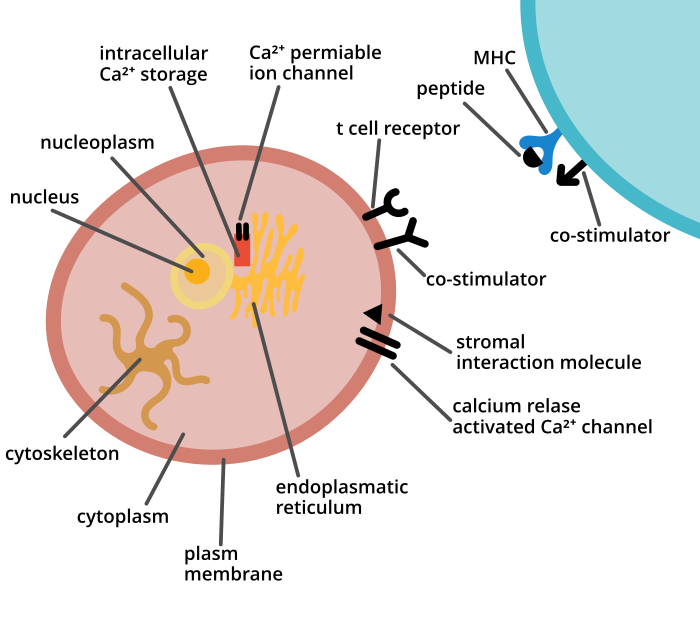
\includegraphics[width=\linewidth]{fig/t_cell_components}
	\caption{Schematic view of a t cell and antigen presenting cell, with all relevant components.}
	\label{fig:tcellcomponents}
\end{figure}

\newpage
\section{Activation of T Cells}
\label{sec:t-cell/activation}

Activation is necessary for t cells to divide and perform their functions.\cite{Ganong1997}

When a native t cell encounters a peptide on an APC that is compatible, a bond is formed between the TCR on the t cell and the peptide-MHC complex on the APC. This recognition can be triggered by less than ten molecules of foreign substance and is therefore described as near perfect. Sufficiently long contact is necessary between the APC and the t cell in order for the t cell to activate. The role of contact time in t cell activation is modelled by Morgan et al.\cite{morgan2023}.

The presence of co-stimulatory molecules is needed for activation. The bond between the co-stimulatory molecules on the t cell and the one on the APC plays a role in signalling. Especially \Calcium signals play a vital part in t cell activation.

An increase of \Calcium in t cells during activation is caused by the stimulation of \Calcium permeable ion channel receptors on the ER membrane. \Calcium is released from the ER into the cytoplasm. Additionally, this decrease in \Calcium is sensed by STIM, which leads to an influx of \Calcium through plasma membrane CRAC channels.\cite{smith2009}

As the intracellular \Calcium concentration is dependent on the interaction between \Calcium sources and sinks, a variety of different forms in \Calcium concentration have been observed. Examples are infrequent spikes, sustained oscillations and plateaus.\cite{Lewis2001}

Intercellular \Calcium increase together with other signals lead to a redistribution of receptors, signalling molecules and organelles.\cite{joseph2014}